\documentclass{article}
\usepackage[utf8]{inputenc}
\usepackage[letterpaper,top=1.5cm,bottom=1.5cm,left=3cm,right=3cm,marginparwidth=1.75cm]{geometry}
\usepackage{natbib}
\usepackage{graphicx}
\usepackage{tikz}
\usepackage{amsmath, amsthm, amssymb, amsfonts}
\usepackage{titlesec}
\usepackage{pdflscape}
\usepackage{makecell}
\usepackage{xcolor,colortbl}
\usepackage{pgfplots}
\usepackage{parskip}
\usetikzlibrary{matrix,chains,positioning,decorations.pathreplacing,arrows}
\usetikzlibrary{positioning,calc}
\usepackage{inconsolata}
\usepackage{neuralnetwork}
\usepackage{xpatch}
\xpatchcmd{\linklayers}{\nn@lastnode}{\lastnode}{}{}
\xpatchcmd{\linklayers}{\nn@thisnode}{\thisnode}{}{}
\usetikzlibrary{shapes}
\tikzset{%
  every neuron/.style={
    circle,
    draw,
    minimum size=1cm
  },
  neuron missing/.style={
    draw=none, 
    scale=2,
    text height=0.333cm,
    execute at begin node=\color{black}$\vdots$
  },
}
\makeatletter
\@addtoreset{subsection}{section}
\makeatother
\def\thesection{Question \arabic{section}}
\def\thesubsection{\arabic{section}. \textit{\alph{subsection}}}
\def\thesubsubsection{\arabic{section}. \textit{\alph{subsection}}. \textit{\roman{subsubsection}}}
\pgfplotsset{compat=1.18}
\title{Artificial Intelligence\\Homework no. 4}
\author{Alireza Rostami\\Student Number: 9832090}
\date{}
\begin{document}
    \maketitle
    \begin{center}
        Find the \LaTeX \ code of this masterpiece at my Github @ github.com/WellOfSorrows.
    \end{center}
    \section{}
    Since in region \textit{A}, the model is too simple, the error is large. Thus, region \textit{A}, corresponds to \textit{under-fitting model complexity}. \par
    In region \textit{B}, the model is of perfect complexity. Thus, region \textit{B} corresponds to \textit{ideal model complexity}. \par
    In region \textit{C}, the model is too complex; thus the error on test data will be greater than model of region \textit{B}. Thus, the region \textit{C} corresponds to \textit{over-fitting model complexity}.
    \section{}
    We use forward propagation to obtain the output and compare it with the actual value to calculate the error.
    
    To minimize the error, we use backward propagation by calculating the derivative of error with respect to each weight and then subtracting this value from the weight value.

    Thus, with forward propagation, we see how well our neural network is performing by calculating the error. Then, we use backward propagation and some sort of a gradient descent to update new values of weights. We again use forward propagation to get the new error, and then use backward propagation to update weights. We will continue this process until we the error reaches some minima.

    \section{}
    There are two types of \textit{perceptrons}: \textit{Single-layer} and \textit{Multi-layer}.
    \begin{itemize}
        \item Single-layer perceptrons: can learn only linearly separable patterns.
        \begin{center}
        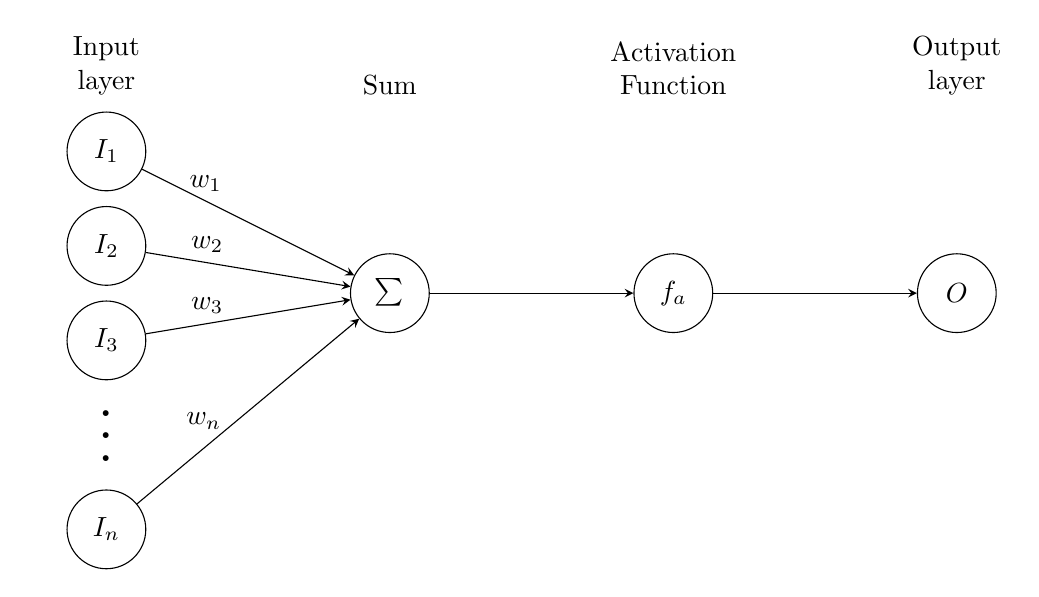
\begin{tikzpicture}[x=1.2cm, y=1.2cm, >=stealth]
        \foreach \m/\l [count=\y] in {1,2,3,missing,4}
            \node [every neuron/.try, neuron \m/.try] (input-\m) at (0,2.5-\y) {};
        \foreach \m [count=\y] in {1}
          \node [every neuron/.try, neuron \m/.try ] (hidden1-\m) at (3,0) {};
         \foreach \m [count=\y] in {1}
          \node [every neuron/.try, neuron \m/.try ] (hidden2-\m) at (6,0) {};
        \foreach \m [count=\y] in {1}
          \node [every neuron/.try, neuron \m/.try ] (output-\m) at (9,0) {};
          
	    \foreach \l [count=\i] in {1,2,3,n}	
            \node at (input-\i) {$I_\l$};	
        \foreach \l [count=\i] in {1}	
            \node at (hidden1-\i) {$\sum_{}^{}$};
        \foreach \l [count=\i] in {1}	
            \node at (hidden2-\i) {$f_a$};	
        \foreach \l [count=\i] in {1}	
            \node at (output-\i) {$O$};
        
        \foreach \i in {1,...,3}
          \foreach \j in {1}
            \draw [->] (input-\i) -- (hidden1-\j) node [pos=0.3, above] {$w_\i$};
        \foreach \i in {4}
          \foreach \j in {1}
            \draw [->] (input-\i) -- (hidden1-\j) node [pos=0.3, above=0.1] {$w_n$};
        \foreach \i in {1}
          \foreach \j in {1}
            \draw [->] (hidden1-\i) -- (hidden2-\j);
        \foreach \i in {1}
          \foreach \j in {1}
            \draw [->] (hidden2-\i) -- (output-\j);
        \node [align=center, above] at (0,2) {Input\\layer};
        \node [align=center, above] at (3,2) {Sum};
        \node [align=center, above] at (6,2) {Activation\\Function};
        \node [align=center, above] at (9,2) {Output\\layer};
        \end{tikzpicture}
        \end{center}

    \item Multi-layer perceptrons (or feedforward neural networks): have two or more layers and thus greater processing power.

        \begin{center}
        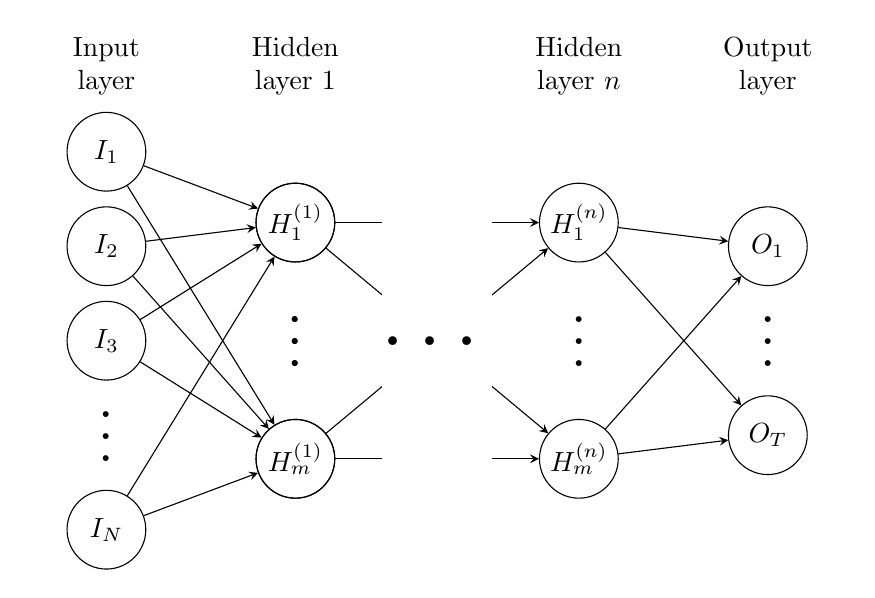
\begin{tikzpicture}[x=1.2cm, y=1.2cm, >=stealth]
        \foreach \m/\l [count=\y] in {1,2,3,missing,4}
            \node [every neuron/.try, neuron \m/.try] (input-\m) at (0,2.5-\y) {};
        \foreach \m [count=\y] in {1,missing,2}
          \node [every neuron/.try, neuron \m/.try ] (hidden1-\m) at (2,2-\y*1.25) {};
        \foreach \m [count=\y] in {1,missing,2}
        \node [every neuron/.try, neuron \m/.try ] (hidden1-\m) at (2,2-\y*1.25) {};
        \foreach \m [count=\y] in {1,missing,2}
          \node [every neuron/.try, neuron \m/.try ] (hidden2-\m) at (5,2-\y*1.25) {};
        \foreach \m [count=\y] in {1,missing,2}
          \node [every neuron/.try, neuron \m/.try ] (output-\m) at (7,1.5-\y) {};
          
	    \foreach \l [count=\i] in {1,2,3,N}	
            \node at (input-\i) {$I_\l$};	
        \foreach \l [count=\i] in {1,m}	
            \node at (hidden1-\i) {$H^{(1)}_\l$};	
        \foreach \l [count=\i] in {1,m}	
            \node at (hidden2-\i) {$H^{(n)}_\l$};	
        \foreach \l [count=\i] in {1,T}	
            \node at (output-\i) {$O_\l$};
        
        \foreach \i in {1,...,4}
          \foreach \j in {1,...,2}
            \draw [->] (input-\i) -- (hidden1-\j);
        \foreach \i in {1,...,2}
          \foreach \j in {1,...,2}
            \draw [->] (hidden1-\i) -- (hidden2-\j);
        \foreach \i in {1,...,2}
          \foreach \j in {1,...,2}
            \draw [->] (hidden2-\i) -- (output-\j);
        \node [align=center, above] at (0,2) {Input\\layer};
        \node [align=center, above] at (2,2) {Hidden \\layer $1$};
        \node [align=center, above] at (5,2) {Hidden \\layer $n$};
        \node [align=center, above] at (7,2) {Output \\layer};
        \node[fill=white,scale=3,inner xsep=0pt,inner ysep=5mm] at ($(hidden1-1)!.5!(hidden2-2)$) {$\dots$};
        \end{tikzpicture}
        \end{center}
    \end{itemize}
    \section{}
    The learning rate controls how fast the model adapts to the problem.
    \begin{itemize}
        \item Smaller learning rates require more training epochs given the smaller changes made to the weights each update. A learning rate that is too small can cause the process to get stuck.
        \item Larger learning rates result in rapid changes and require fewer training epochs. A learning rate that is too large can cause the model to converge too quickly to a suboptimal solution.
    \end{itemize}
\end{document}
